%% ====================================================================
%%  Subseasonal Forecast Skill over India:
%%  A Two-Season Benchmark of AI-Based and Operational Models
%%
%%  arXiv-style single-column preprint  --  STRUCTURED SCAFFOLD (v0)
%% --------------------------------------------------------------------
%%  BUILD CONTRACT
%%   * Structure built with Opus; prose to be expanded/polished with Sonnet.
%%   * Every \TODO{...} marks prose work to be done. Search "\TODO".
%%   * ALL numbers come from tables/*.tex and figs/*.pdf, which are
%%     regenerated from the result CSVs by:
%%         python scripts/make_tables.py
%%         python scripts/make_figures.py
%%     Do NOT hand-type scores; edit the scripts and rerun.
%%   * Compile:  tectonic s2s_india_benchmark.tex   (run inside tectonic_env)
%% ====================================================================
\documentclass[11pt,a4paper]{article}

%% --- fonts & encoding ---------------------------------------------------
\usepackage[utf8]{inputenc}
\usepackage[T1]{fontenc}
\usepackage{lmodern}
\usepackage{microtype}

%% --- layout -------------------------------------------------------------
\usepackage[a4paper,margin=1in]{geometry}
\usepackage{setspace}
\onehalfspacing

%% --- math, tables, figures ----------------------------------------------
\usepackage{amsmath,amssymb}
\usepackage{graphicx}
\usepackage{booktabs}
\usepackage{multirow}
\usepackage{array}
\usepackage[font=small,labelfont=bf]{caption}

%% --- bibliography & links -----------------------------------------------
\usepackage[round,authoryear]{natbib}
\usepackage{xcolor}
\definecolor{linkblue}{RGB}{30,80,160}
\usepackage[colorlinks=true,linkcolor=linkblue,citecolor=linkblue,
            urlcolor=linkblue]{hyperref}
\providecommand{\doi}[1]{\href{https://doi.org/#1}{doi:#1}}

%% --- review aids --------------------------------------------------------
\usepackage{lineno}
% \linenumbers   % uncomment for review copies
\newcommand{\TODO}[1]{\textcolor{red}{[\textbf{TODO:} #1]}}
\newcommand{\ph}[1]{\textcolor{red}{[#1]}}

\title{\vspace{-1.0cm}\bfseries
  Subseasonal Forecast Skill over India: A Two-Season Benchmark of
  AI-Based and Operational Models}

\author{%
  Ayush Raj Tamta$^{1,2}$, Manmeet Singh$^{3}$, Saptarishi Dhanuka$^{1}$,\\
  Parthasarathi Mukhopadhyay$^{1}$, Bedartha Goswami$^{2}$, Sandeep Juneja$^{1}$\\[0.4em]
  \small $^{1}$Ashoka University, India \quad
  $^{2}$IISER Pune, India \quad
  $^{3}$Western Kentucky University, USA\\
  \small\texttt{raj.ayush@students.iiserpune.ac.in}
}
\date{\today}

\begin{document}
\maketitle

% ======================================================================
\begin{abstract}
\noindent
\TODO{Final abstract pass. Skeleton below states the three findings; tighten
to $\sim$200 words and add one quantitative hook per finding.}

Subseasonal-to-seasonal (S2S) prediction at two-to-six-week leads is of high
value for Indian agriculture and water management, yet precipitation skill at
these leads is limited and the performance of new machine-learning (ML)
forecast systems over India is largely undocumented. We benchmark six S2S
systems---three ML-based (Spire AI-S2S, FuXi-S2S, DLESyM) and three
operational dynamical (ECMWF, UKMO, NCEP)---for weekly precipitation, 500-hPa
geopotential height (Z500), and 2-m temperature (T2M) over India across two
contrasting seasons: the synoptically driven winter (JFM~2026, 90 daily
initializations) and the convectively dominated summer monsoon (JJAS~2019, 17
common initializations). Forecasts are verified against ERA5 (Z500, T2M),
ERA5 daily totals and IMD gridded rainfall (precipitation), using
cosine-weighted ACC, RMSE, bias, and a common probabilistic framework (CRPSS,
spread--skill ratio). We report three findings. (i)~In winter, the ML system
Spire AI-S2S is the most skillful system for precipitation at every lead
(week-1 ACC~0.78 versus 0.73 for ECMWF) and uniquely retains Z500 skill to
week~6, whereas the other two ML systems (FuXi-S2S, DLESyM) lose all Z500
skill---falling to negative ACC---by week~3--4. (ii)~In the monsoon, this ML
advantage disappears: every system, ML and dynamical alike, loses
precipitation skill by week~3 (all-India ACC~$\le$~0.06 at week~3). (iii)~The
deterministic ranking does not carry over to probabilistic skill: ECMWF leads
precipitation CRPSS despite Spire's higher ACC. These results give an early,
honest assessment of where ML S2S systems help over India and where the
problem remains hard for all approaches.
\end{abstract}

\vspace{0.3em}
\noindent\textbf{Keywords:} subseasonal-to-seasonal prediction; machine
learning; precipitation; India; monsoon; ensemble verification

% ======================================================================
\section{Introduction}\label{sec:intro}

% Paragraph 1 -- why S2S over India matters
\TODO{Expand. Topic sentence + societal motivation (rabi crops, water, WDs,
monsoon). Reuse prose from the prior draft's Introduction.}
Subseasonal-to-seasonal (S2S) prediction bridges medium-range weather and
seasonal climate forecasting and is increasingly demanded for Indian
agriculture, water resources, and disaster preparedness
\citep{vitart2017,white2017,mariotti2020}.

% Paragraph 2 -- the rise of ML forecasting and the gap
\TODO{Expand. ML weather models now rival NWP at medium range; extension to
S2S is recent (FuXi-S2S); regional precip skill over India undocumented.
Reuse Intro \P3.}
Machine-learning (ML) forecast systems now match or exceed operational
numerical weather prediction (NWP) at medium range
\citep{pathak2022,bi2023,lam2023,benbouallegue2024}, and their extension to
the subseasonal range has begun \citep{chen2024,spire2026}.

% Paragraph 3 -- the two-season framing (the novelty of THIS paper)
\TODO{Expand into the paper's central idea. Key argument: a single season
cannot separate "ML is better" from "ML is better at easy regimes." We test
two regimes deliberately --- winter (synoptic, WD-driven, higher
predictability) vs monsoon (convective, lower S/N) --- to find WHERE ML helps.}
A single-season benchmark cannot distinguish a genuinely better forecast
system from one that merely performs well in an easy regime. We therefore
evaluate the same six systems across two physically contrasting seasons over
the same domain.

% Paragraph 4 -- contributions / questions
We address four questions:
\begin{enumerate}\setlength{\itemsep}{1pt}
  \item How does weekly skill for precipitation, Z500, and T2M decay with lead
        time (weeks~1--6) for each system, in winter and in the monsoon?
  \item Do ML systems outperform operational dynamical systems over India, and
        does any advantage persist across both seasons?
  \item Do the ML systems behave consistently with one another, or do they
        diverge at long lead?
  \item Does deterministic skill translate into probabilistic (calibrated)
        skill?
\end{enumerate}

\TODO{Close Intro with a one-paragraph roadmap of the paper.}

% ======================================================================
\section{Data and Study Domain}\label{sec:data}

\subsection{Study domain and regions}\label{sec:domain}
\TODO{Domain box 5--38N, 65--100E; land points only; cosine weights; four IMD
homogeneous regions (Northwest, Central, South Peninsula, East/NE). Reuse
Domain subsection + Fig.~domain from old paper. Add region map figure.}

\subsection{Verification references}\label{sec:truth}
\TODO{Describe the three truth sources and WHY each is used.}
\begin{itemize}\setlength{\itemsep}{1pt}
  \item \textbf{Precipitation, winter:} ERA5 daily totals (00--00\,UTC),
        \TODO{cite ARCO-ERA5 carver2023; note IMD-2026 not yet available.}
  \item \textbf{Precipitation, monsoon:} IMD $0.25^\circ$ gauge-based gridded
        rainfall \citep{pai2014} --- an observational reference independent of
        any reanalysis.
  \item \textbf{Z500 and T2M:} ERA5 \citep{hersbach2020}; for JJAS the local
        WeatherBench2 ERA5 archive \citep{rasp2024}.
\end{itemize}

\subsection{Forecast systems}\label{sec:models_data}
\TODO{One short paragraph; details in Table~\ref{tab:models} and
Sec.~\ref{sec:models}.}
\begin{table}[t]
  \centering
  \caption{Forecast systems evaluated. ``Native res.'' is each model's own
  horizontal grid; all are regridded to the common $1.5^\circ$ verification
  grid before scoring. CF\,=\,control, PF\,=\,perturbed member. ``Both'' =
  evaluated in JFM\,2026 and JJAS\,2019.}
  \label{tab:models}
  \small
  \begin{tabular}{llcccc}
    \toprule
    System & Type & Native res. & Members & Horizon & Seasons \\
    \midrule
    Spire AI-S2S & ML (data-driven)    & $0.5^\circ$        & mean+s.d. & 46\,d & JFM\,2026 \\
    FuXi-S2S     & ML (transformer)    & $1.5^\circ$        & 1CF+10PF  & 42\,d & Both \\
    DLESyM       & ML (diffusion)      & $0.25^\circ$       & 80\,PF    & 48\,d & Both \\
    ECMWF        & Dynamical, coupled  & Tco319 ($\sim$36\,km) & 100\,PF & 46\,d & Both \\
    UKMO GloSea6 & Dynamical, coupled  & N216 ($\sim$60\,km)   & 1CF+3PF & 60\,d & Both \\
    NCEP CFSv2   & Dynamical, coupled  & T126 ($\sim$100\,km)  & 15\,PF  & 44\,d & Both \\
    \bottomrule
  \end{tabular}
\end{table}
   % hand-written model table (see note below)

% ======================================================================
\section{Forecast Systems}\label{sec:models}
\TODO{One subsection each. Keep to 4--6 sentences: lineage, resolution,
ensemble, how each variable is delivered + unit handling. Reuse ECMWF/NCEP/
Spire/FuXi text from old paper; write UKMO + DLESyM fresh (see notes).}

\subsection{Spire AI-S2S}\label{sec:spire}
\TODO{ML, $0.5^\circ$, mean+s.d., 46\,d, ERA5-initialized, daily TP (no unit
conv).}

\subsection{FuXi-S2S}\label{sec:fuxi}
\TODO{ML transformer, $1.5^\circ$, 1CF+10PF, 42\,d, TP delivered as mm\,h$^{-1}$
$\Rightarrow\times24$.}

\subsection{DLESyM}\label{sec:delysm}
\TODO{Diffusion-based ML, $0.25^\circ$, 80 members, 48\,d, 6-hourly
$\Rightarrow$ daily-mean; z500 geopotential $\div g$; NO precipitation channel
(Z500/T2M only). Note 3 corrupted stores excluded.}

\subsection{ECMWF extended-range ensemble}\label{sec:ecmwf}
\TODO{IFS, Tco319, 100PF, 46\,d; cumulative TP $\Rightarrow$ de-accumulate.}

\subsection{UKMO GloSea6}\label{sec:ukmo}
\TODO{MetUM, N216, 1CF+3PF, 60\,d; cumulative TP; z500 already gpm; T2M broken
(single lead) $\Rightarrow$ excluded from rankings.}

\subsection{NCEP CFSv2}\label{sec:ncep}
\TODO{T126, 15PF, 44\,d; cumulative TP.}

% ======================================================================
\section{Verification Framework}\label{sec:methods}

\subsection{Weekly lead windows and aggregation}\label{sec:weeks}
\TODO{Day-1 = first 24\,h after init; W1=days1--7 \dots W6=days36--42; weekly
means; common $1.5^\circ$ grid; cosine-lat weights; land mask.}

\subsection{Anomalies and climatology}\label{sec:anom}
\TODO{ERA5 1990--2019 day-of-year climatology for Z500/T2M and ERA5-truth TP;
IMD 1991--2020 daily climatology for IMD-truth TP. Common climatology removed
identically from forecast and truth.}

\subsection{Deterministic and probabilistic metrics}\label{sec:metrics}
\TODO{Define ACC (cosine-weighted), RMSE, bias, MAE; then CRPS, CRPSS vs
climatology, spread--skill ratio; Brier for TP exceedance events. Equations
can be lifted from old paper Sec.~Metrics.}

\subsection{Initialization sets and matched comparison}\label{sec:inits}
\TODO{Explain the two init sets explicitly --- this is a methods strength:}
\begin{itemize}\setlength{\itemsep}{1pt}
  \item \textbf{JFM~2026:} 90 daily 00\,UTC initializations
        (1~Jan--31~Mar~2026). \TODO{note W5/W6 sample shrinks as ERA5 truth
        ends 31~Mar.}
  \item \textbf{JJAS~2019:} 17 common Thursday initializations
        (6~Jun--26~Sep~2019) on which all five non-Spire models provide usable
        forecasts; this matched set is the basis of all cross-model JJAS
        comparisons. A 35-initialization operational subset (ECMWF, UKMO,
        NCEP) is used as a robustness check (Sec.~\ref{sec:robust}).
\end{itemize}

% ======================================================================
\section{Results}\label{sec:results}

\subsection{Overview: skill across variables and seasons}\label{sec:overview}
Figure~\ref{fig:acc_lead} summarizes the whole benchmark: anomaly correlation
versus lead week for all six systems, three variables, and both seasons.
\TODO{Walk the reader through the figure in 4--5 sentences, foreshadowing the
three findings (winter ML advantage; monsoon collapse; ML divergence).}

\begin{figure}[t]
  \centering
  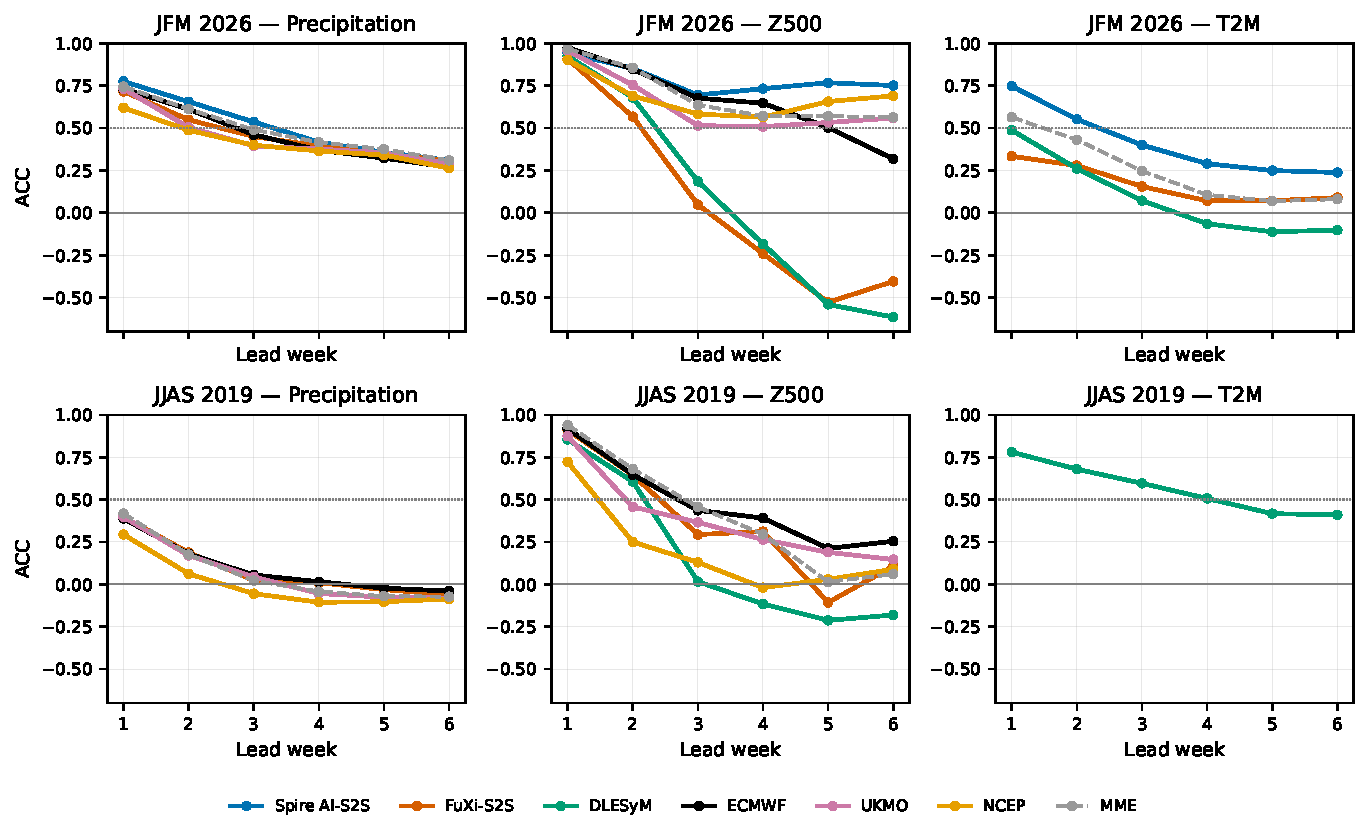
\includegraphics[width=\linewidth]{figs/fig_acc_lead.pdf}
  \caption{All-India anomaly correlation (ACC) versus lead week for six S2S
  systems. Top row: JFM~2026 (winter); bottom row: JJAS~2019 (monsoon).
  Columns: precipitation, Z500, 2-m temperature. Dotted line ACC$=0.5$; solid
  line ACC$=0$. DLESyM provides no precipitation; UKMO T2M and Spire (JJAS)
  are unavailable.}
  \label{fig:acc_lead}
\end{figure}

\subsection{Winter (JFM 2026): the ML advantage}\label{sec:jfm}
\TODO{Lead with precipitation. SPIRE best at every lead (W1 0.78 vs 0.73
ECMWF/UKMO, 0.62 NCEP; lowest RMSE 1.09 mm/day, near-zero bias -0.04). Then
Z500: SPIRE holds 0.69--0.77 W3--W6 while FuXi/DLESyM go NEGATIVE. Then T2M:
SPIRE dominant. Cite the three ACC tables + RMSE table.}
\begin{table}[t]
  \centering
  \caption{JFM~2026 all-India precipitation anomaly correlation (ACC) by lead week, verified against ERA5 daily totals. Best individual-model score in each column is bold; MME is the multi-model mean.}
  \label{tab:jfm_acc_tp}
  \small
  \begin{tabular}{lcccccc}
    \toprule
    Model & W1 & W2 & W3 & W4 & W5 & W6 \\
    \midrule
    Spire AI-S2S   & $\mathbf{0.78}$ & $\mathbf{0.66}$ & $\mathbf{0.54}$ & $\mathbf{0.42}$ & $\mathbf{0.36}$ & $\mathbf{0.31}$ \\
FuXi-S2S       & $0.72$ & $0.55$ & $0.45$ & $0.39$ & $0.35$ & $0.31$ \\
ECMWF          & $0.73$ & $0.61$ & $0.46$ & $0.37$ & $0.32$ & $0.27$ \\
UKMO           & $0.73$ & $0.50$ & $0.39$ & $0.38$ & $0.35$ & $0.28$ \\
NCEP           & $0.62$ & $0.49$ & $0.40$ & $0.36$ & $0.34$ & $0.26$ \\
MME            & $0.74$ & $0.61$ & $0.49$ & $0.42$ & $0.37$ & $0.31$ \\
    \bottomrule
  \end{tabular}
\end{table}

\begin{table}[t]
  \centering
  \caption{JFM~2026 all-India Z500 ACC by lead week (ERA5 truth).}
  \label{tab:jfm_acc_z500}
  \small
  \begin{tabular}{lcccccc}
    \toprule
    Model & W1 & W2 & W3 & W4 & W5 & W6 \\
    \midrule
    Spire AI-S2S   & 0.94 & \textbf{0.85} & \textbf{0.69} & \textbf{0.73} & \textbf{0.77} & \textbf{0.75} \\
FuXi-S2S       & 0.91 & 0.57 & 0.05 & -0.24 & -0.53 & -0.40 \\
DLESyM         & 0.92 & 0.68 & 0.19 & -0.18 & -0.54 & -0.62 \\
ECMWF          & \textbf{0.97} & 0.85 & 0.68 & 0.65 & 0.50 & 0.32 \\
UKMO           & 0.96 & 0.75 & 0.51 & 0.51 & 0.53 & 0.56 \\
NCEP           & 0.90 & 0.69 & 0.58 & 0.56 & 0.66 & 0.69 \\
MME            & 0.97 & 0.86 & 0.64 & 0.57 & 0.57 & 0.56 \\
    \bottomrule
  \end{tabular}
\end{table}

\begin{table}[t]
  \centering
  \caption{JFM~2026 all-India 2-m temperature ACC by lead week (ERA5 truth).}
  \label{tab:jfm_acc_t2m}
  \small
  \begin{tabular}{lcccccc}
    \toprule
    Model & W1 & W2 & W3 & W4 & W5 & W6 \\
    \midrule
    Spire AI-S2S   & \textbf{0.75} & \textbf{0.55} & \textbf{0.40} & \textbf{0.29} & \textbf{0.25} & \textbf{0.24} \\
FuXi-S2S       & 0.33 & 0.28 & 0.16 & 0.07 & 0.07 & 0.09 \\
DLESyM         & 0.49 & 0.26 & 0.07 & -0.06 & -0.11 & -0.10 \\
MME            & 0.56 & 0.43 & 0.25 & 0.11 & 0.07 & 0.08 \\
    \bottomrule
  \end{tabular}
\end{table}

\begin{table}[t]
  \centering
  \caption{JFM~2026 all-India precipitation RMSE (mm\,day$^{-1}$) by lead week.}
  \label{tab:jfm_rmse_tp}
  \small
  \begin{tabular}{lcccccc}
    \toprule
    Model & W1 & W2 & W3 & W4 & W5 & W6 \\
    \midrule
    Spire AI-S2S   & $\mathbf{1.09}$ & $\mathbf{1.44}$ & $\mathbf{1.68}$ & $\mathbf{1.88}$ & $\mathbf{2.14}$ & $\mathbf{2.28}$ \\
FuXi-S2S       & $1.33$ & $1.83$ & $1.95$ & $2.08$ & $2.34$ & $2.47$ \\
ECMWF          & $1.27$ & $1.59$ & $1.92$ & $2.14$ & $2.40$ & $2.57$ \\
UKMO           & $1.31$ & $1.90$ & $2.16$ & $2.14$ & $2.36$ & $2.56$ \\
NCEP           & $1.57$ & $1.93$ & $2.15$ & $2.29$ & $2.49$ & $2.75$ \\
MME            & $1.18$ & $1.54$ & $1.80$ & $1.94$ & $2.18$ & $2.35$ \\
    \bottomrule
  \end{tabular}
\end{table}


\subsection{Monsoon (JJAS 2019): the great equalizer}\label{sec:jjas}
\TODO{Key message: ALL systems collapse. Precip W1 ~0.4 (0.29 NCEP) -> <=0.06
by W3 -> negative after. No ML advantage. Z500 horizon also shorter than
winter. DLESyM Z500 collapses fastest; ECMWF/UKMO most persistent. T2M only
DLESyM available (0.78->0.41). Cite JJAS tables.}
\begin{table}[t]
  \centering
  \caption{JJAS~2019 all-India precipitation ACC by lead week, verified against IMD gridded rainfall (17 common initializations).}
  \label{tab:jjas_acc_tp}
  \small
  \begin{tabular}{lcccccc}
    \toprule
    Model & W1 & W2 & W3 & W4 & W5 & W6 \\
    \midrule
    FuXi-S2S       & 0.40 & \textbf{0.19} & 0.02 & 0.01 & -0.03 & -0.06 \\
ECMWF          & 0.39 & 0.18 & \textbf{0.06} & \textbf{0.02} & \textbf{-0.02} & \textbf{-0.04} \\
UKMO           & \textbf{0.40} & 0.17 & 0.04 & -0.05 & -0.08 & -0.08 \\
NCEP           & 0.29 & 0.06 & -0.05 & -0.11 & -0.10 & -0.09 \\
MME            & 0.42 & 0.18 & 0.02 & -0.04 & -0.07 & -0.07 \\
    \bottomrule
  \end{tabular}
\end{table}

\begin{table}[t]
  \centering
  \caption{JJAS~2019 all-India Z500 ACC by lead week (ERA5 truth, 17 common initializations).}
  \label{tab:jjas_acc_z500}
  \small
  \begin{tabular}{lcccccc}
    \toprule
    Model & W1 & W2 & W3 & W4 & W5 & W6 \\
    \midrule
    FuXi-S2S       & 0.91 & 0.64 & 0.29 & 0.31 & -0.11 & 0.11 \\
DLESyM         & 0.85 & 0.61 & 0.02 & -0.12 & -0.21 & -0.18 \\
ECMWF          & \textbf{0.92} & \textbf{0.65} & \textbf{0.44} & \textbf{0.39} & \textbf{0.21} & \textbf{0.25} \\
UKMO           & 0.87 & 0.46 & 0.37 & 0.26 & 0.19 & 0.15 \\
NCEP           & 0.72 & 0.25 & 0.13 & -0.02 & 0.03 & 0.09 \\
MME            & 0.94 & 0.68 & 0.46 & 0.30 & 0.01 & 0.06 \\
    \bottomrule
  \end{tabular}
\end{table}


\subsection{Divergence among the ML systems}\label{sec:ml_divergence}
\TODO{Dedicated subsection making finding (iii) explicit: SPIRE vs
FuXi/DLESyM. At W1 all three ML look comparable; by W3--4 SPIRE is flat while
FuXi+DLESyM Z500 ACC < 0. Argue this is a long-lead stability / error-growth
property, not a headline-score property --- a caution against ranking ML
systems on week-1 numbers alone. Reference Fig.~\ref{fig:acc_lead} middle
column.}

\subsection{Probabilistic skill and calibration}\label{sec:prob}
\TODO{The "deterministic != probabilistic" finding. ECMWF leads TP CRPSS
(0.59 W1) over SPIRE (0.61 W1 actually ties --- CHECK and state precisely);
for Z500 ECMWF leads early but SPIRE most persistent. Spread-skill: who is
under/over-dispersive. Cite CRPSS tables + spread-skill figure.}
\begin{table}[t]
  \centering
  \caption{JFM~2026 all-India precipitation CRPSS versus climatology by lead week. Positive values indicate probabilistic skill above climatology.}
  \label{tab:jfm_crpss_tp}
  \small
  \begin{tabular}{lcccccc}
    \toprule
    Model & W1 & W2 & W3 & W4 & W5 & W6 \\
    \midrule
    Spire AI-S2S   & $\mathbf{0.61}$ & $0.40$ & $0.25$ & $0.19$ & $0.18$ & $0.17$ \\
FuXi-S2S       & $0.45$ & $0.27$ & $0.31$ & $0.32$ & $0.29$ & $\mathbf{0.26}$ \\
ECMWF          & $0.59$ & $\mathbf{0.51}$ & $\mathbf{0.40}$ & $\mathbf{0.35}$ & $\mathbf{0.30}$ & $0.25$ \\
UKMO           & $0.45$ & $0.27$ & $0.18$ & $0.25$ & $0.23$ & $0.18$ \\
NCEP           & $0.42$ & $0.33$ & $0.29$ & $0.26$ & $0.24$ & $0.14$ \\
    \bottomrule
  \end{tabular}
\end{table}

\begin{table}[t]
  \centering
  \caption{JFM~2026 all-India Z500 CRPSS versus climatology by lead week.}
  \label{tab:jfm_crpss_z500}
  \small
  \begin{tabular}{lcccccc}
    \toprule
    Model & W1 & W2 & W3 & W4 & W5 & W6 \\
    \midrule
    Spire AI-S2S   & 0.59 & 0.41 & 0.28 & \textbf{0.28} & \textbf{0.30} & \textbf{0.29} \\
FuXi-S2S       & 0.71 & 0.04 & -0.26 & -0.27 & -0.02 & 0.13 \\
DLESyM         & 0.56 & 0.34 & 0.09 & -0.05 & 0.07 & 0.10 \\
ECMWF          & \textbf{0.83} & \textbf{0.58} & \textbf{0.37} & 0.23 & 0.23 & 0.23 \\
UKMO           & 0.77 & 0.32 & 0.10 & 0.13 & 0.13 & 0.13 \\
NCEP           & 0.26 & -0.19 & -0.18 & -0.13 & 0.02 & 0.02 \\
    \bottomrule
  \end{tabular}
\end{table}


\begin{figure}[t]
  \centering
  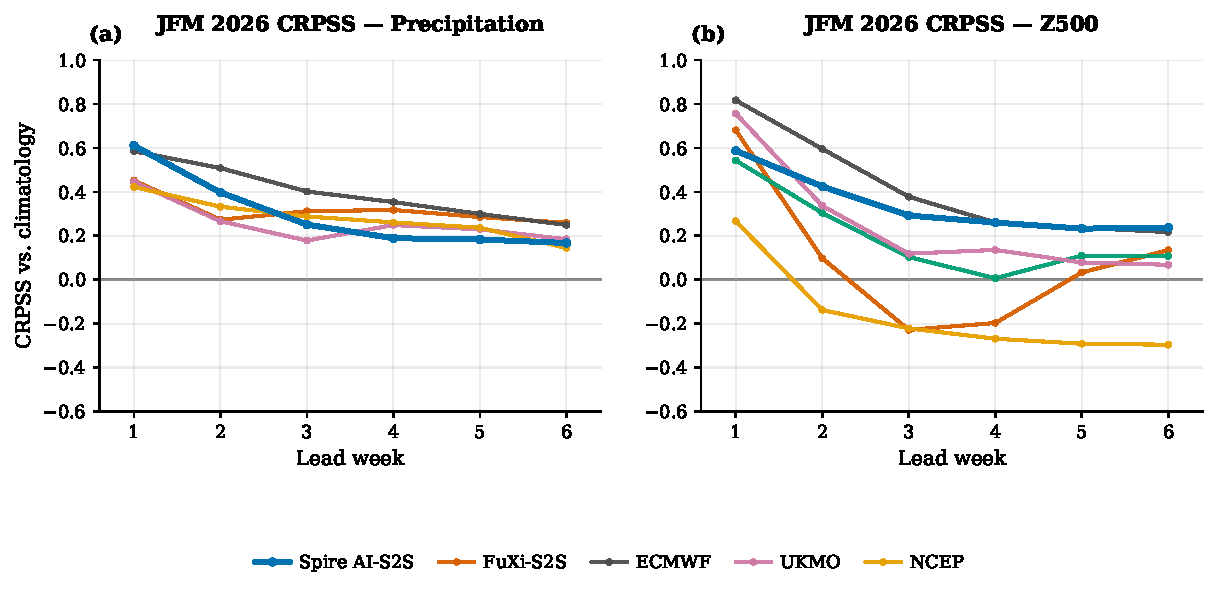
\includegraphics[width=\linewidth]{figs/fig_crpss.pdf}
  \caption{JFM~2026 all-India CRPSS versus lead week for precipitation (left)
  and Z500 (right). Positive values indicate probabilistic skill above
  climatology.}
  \label{fig:crpss}
\end{figure}

\begin{figure}[t]
  \centering
  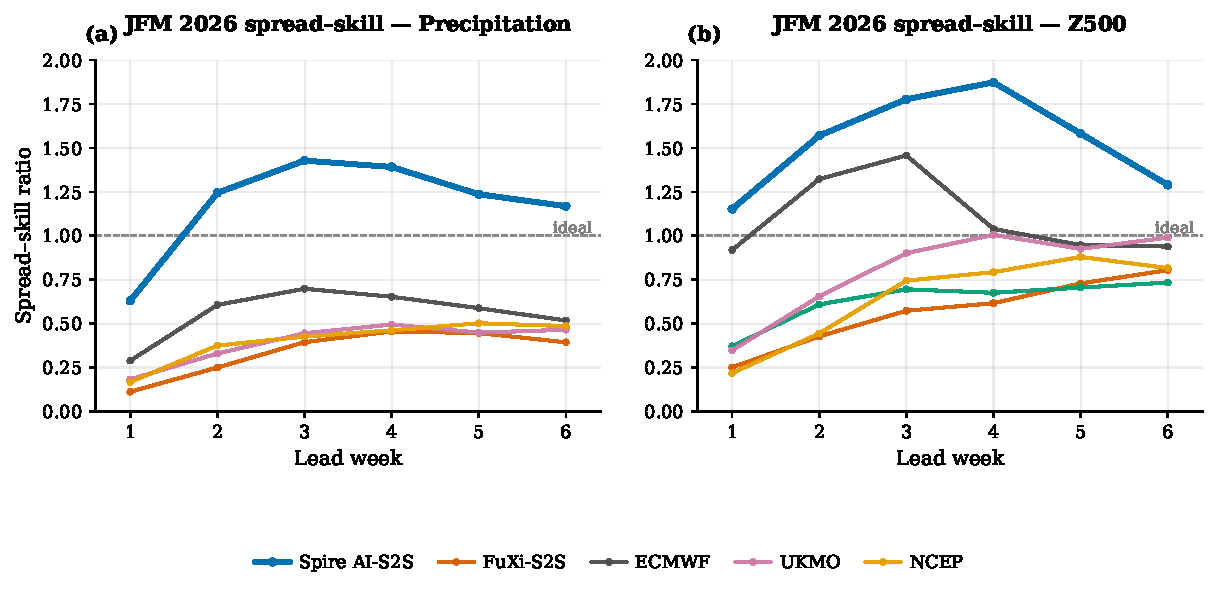
\includegraphics[width=\linewidth]{figs/fig_spread_skill.pdf}
  \caption{JFM~2026 spread--skill ratio versus lead week; a well-calibrated
  ensemble lies near unity (dashed line). Values $<1$ indicate
  under-dispersion (overconfidence).}
  \label{fig:spread_skill}
\end{figure}

\subsection{Regional structure of skill}\label{sec:regional}
\TODO{Use the scorecard: which IMD regions are most/least predictable in
winter; does SPIRE's lead hold in all four regions. 3--4 sentences.}
\begin{figure}[t]
  \centering
  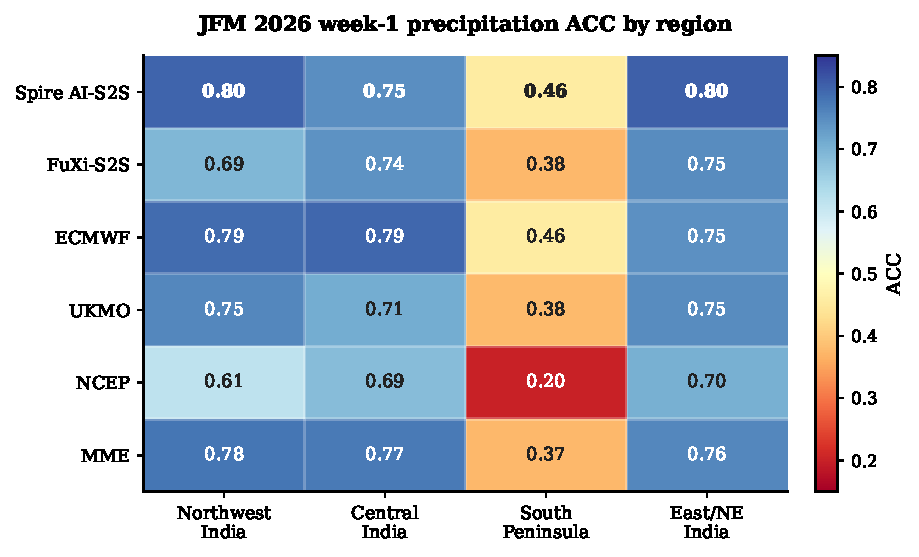
\includegraphics[width=0.8\linewidth]{figs/fig_regional_scorecard.pdf}
  \caption{JFM~2026 week-1 precipitation ACC by IMD homogeneous region.}
  \label{fig:scorecard}
\end{figure}

\subsection{Robustness: larger initialization set}\label{sec:robust}
\TODO{State that the JJAS conclusions are unchanged on the 35-init operational
subset (ECMWF/UKMO/NCEP), confirming the monsoon collapse is not an artifact
of the 17-init matched set. Optionally a small table or one sentence with
numbers from the 35-init operational runs.}

% ======================================================================
\section{Discussion}\label{sec:discussion}

\paragraph{Where ML helps, and where it does not.}
\TODO{Synthesize findings (i)+(ii): ML's winter advantage is real but
regime-dependent; the monsoon remains hard for all systems. Tie to
predictability of synoptic (WD) vs convective regimes.}

\paragraph{Not all AI systems are equal.}
\TODO{Finding (iii): long-lead stability differs sharply across ML systems;
caution against single-lead leaderboard rankings; hypothesize causes
(training objective / error growth in transformer vs diffusion vs Spire).}

\paragraph{Deterministic vs probabilistic skill.}
\TODO{Finding (iv): calibration is a distinct axis; ECMWF's mature ensemble
still leads probabilistically. Operational guidance should weigh both.}

\paragraph{Comparison with prior S2S literature.}
\TODO{Consistency with deandrade2019 / South-Asia S2S: precip skill to ~week 2;
circulation horizon longer. Cite.}

% ======================================================================
\section{Limitations}\label{sec:limitations}
\TODO{Honest list: (a) two seasons / different years --- not a multi-year
hindcast; (b) JFM uses ERA5 precip truth (IMD-2026 unavailable) while JJAS
uses IMD --- truth differs between seasons; (c) Spire absent in 2019;
(d) common ERA5 climatology, no per-model bias correction; (e) small ensembles
for UKMO (4) limit its probabilistic scores; (f) UKMO T2M and DLESyM precip
unavailable; (g) FuXi T2M has a known $\sim$4\,K cold offset (00\,UTC snapshot
vs daily-mean), reported but not corrected.}

% ======================================================================
\section{Conclusions}\label{sec:conclusions}
\TODO{Restate the three+one findings crisply as numbered takeaways; end with
the reproducible-framework sentence and outlook (more seasons, IMD-2026 truth,
per-model climatology).}

% ======================================================================
\section*{Data and Code Availability}
\TODO{ERA5/ARCO; IMD \citep{pai2014}; ECMWF/UKMO/NCEP via S2S database
\citep{vitart2017}; FuXi-S2S weights (Zenodo/GitHub); Spire under research
agreement; DLESyM via provider. Analysis code:
\url{https://github.com/Artamta/s2s-analysis}.}

\section*{Acknowledgements}
\TODO{Reuse from old paper; A.R.T.\ MSc thesis at IISER Pune; HPC; provider
acknowledgements; LLM-assistance disclosure.}

% ======================================================================
% Bibliography (32 entries carried over from the prior draft).
\begin{thebibliography}{99}

\bibitem[{Ben~Bouall\`egue et~al.(2024)}]{benbouallegue2024}
Ben~Bouall\`egue, Z., and Coauthors, 2024: The rise of data-driven
weather forecasting: A first statistical assessment of machine
learning--based weather forecasts in an operational-like context.
\textit{Bull. Amer. Meteor. Soc.}, \textbf{105}, E864--E883,
\doi{10.1175/BAMS-D-23-0162.1}.

\bibitem[{Bi et~al.(2023)}]{bi2023}
Bi, K., L. Xie, H. Zhang, X. Chen, X. Gu, and Q. Tian, 2023: Accurate
medium-range global weather forecasting with 3D neural networks.
\textit{Nature}, \textbf{619}, 533--538.

\bibitem[{Carver and Merose(2023)}]{carver2023}
Carver, R., and A. Merose, 2023: ARCO-ERA5: An Analysis-Ready,
Cloud-Optimized reanalysis dataset. \textit{Proc.\ 22nd Conf.\ on
Artificial Intelligence for Environmental Science}, Denver, CO,
Amer.\ Meteor.\ Soc., Paper 4A.1.

\bibitem[{Chen et~al.(2024)}]{chen2024}
Chen, L., X. Zhong, H. Li, J. Wu, B. Lu, D. Chen, S.-P. Xie, L. Wu,
Q. Chao, C. Lin, Z. Hu, and Y. Qi, 2024: A machine learning model
that outperforms conventional global subseasonal forecast models.
\textit{Nat. Commun.}, \textbf{15}, 6425,
\doi{10.1038/s41467-024-50714-1}.

\bibitem[{Cresswell-Clay et~al.(2025)}]{cresswellclay2024}
Cresswell-Clay, N., and Coauthors, 2025: A deep learning Earth system
model for efficient simulation of the observed climate.
\textit{AGU Adv.}, \textbf{6}, e2025AV001706,
\doi{10.1029/2025AV001706}.

\bibitem[{de~Andrade et~al.(2019)}]{deandrade2019}
de~Andrade, F.~M., C.~A.~S. Coelho, and I.~F.~A. Cavalcanti, 2019:
Global precipitation hindcast quality assessment of the Subseasonal
to Seasonal (S2S) prediction project models. \textit{Climate Dyn.},
\textbf{52}, 5451--5475.

\bibitem[{Dimri et~al.(2015)}]{dimri2015}
Dimri, A.~P., D. Niyogi, A.~P. Barros, J. Ridley, U.~C. Mohanty,
T. Yasunari, and D.~R. Sikka, 2015: Western disturbances: A review.
\textit{Rev. Geophys.}, \textbf{53}, 225--246.

\bibitem[{Domeisen et~al.(2022)}]{domeisen2022}
Domeisen, D.~I.~V., and Coauthors, 2022: Advances in the subseasonal
prediction of extreme events: Relevant case studies across the globe.
\textit{Bull. Amer. Meteor. Soc.}, \textbf{103}, E1473--E1501,
\doi{10.1175/BAMS-D-20-0221.1}.

\bibitem[{Gneiting and Raftery(2007)}]{gneiting2007}
Gneiting, T., and A.~E. Raftery, 2007: Strictly proper scoring rules,
prediction, and estimation. \textit{J. Amer. Statist. Assoc.},
\textbf{102}, 359--378.

\bibitem[{Hersbach et~al.(2020)}]{hersbach2020}
Hersbach, H., and Coauthors, 2020: The ERA5 global reanalysis.
\textit{Quart. J. Roy. Meteor. Soc.}, \textbf{146}, 1999--2049.

\bibitem[{Hunt et~al.(2018)}]{hunt2018}
Hunt, K.~M.~R., A.~G. Turner, and L.~C. Shaffrey, 2018: The evolution,
seasonality and impacts of western disturbances. \textit{Quart. J.
Roy. Meteor. Soc.}, \textbf{144}, 278--290.

\bibitem[{Kochkov et~al.(2024)}]{kochkov2024}
Kochkov, D., and Coauthors, 2024: Neural general circulation models
for weather and climate. \textit{Nature}, \textbf{632}, 1060--1066.

\bibitem[{Lam et~al.(2023)}]{lam2023}
Lam, R., and Coauthors, 2023: Learning skillful medium-range global
weather forecasting. \textit{Science}, \textbf{382}, 1416--1421.

\bibitem[{Lang et~al.(2024)}]{lang2024}
Lang, S., and Coauthors, 2024: AIFS---ECMWF's data-driven forecasting
system. arXiv preprint, arXiv:2406.01465.

\bibitem[{Mariotti et~al.(2020)}]{mariotti2020}
Mariotti, A., and Coauthors, 2020: Windows of opportunity for skillful
forecasts subseasonal to seasonal and beyond. \textit{Bull. Amer.
Meteor. Soc.}, \textbf{101}, E608--E625.

\bibitem[{Murphy(1988)}]{murphy1988}
Murphy, A.~H., 1988: Skill scores based on the mean square error and
their relationships to the correlation coefficient. \textit{Mon. Wea.
Rev.}, \textbf{116}, 2417--2424.

\bibitem[{National Academies(2016)}]{nas2016}
National Academies of Sciences, Engineering, and Medicine, 2016:
\textit{Next Generation Earth System Prediction: Strategies for
Subseasonal to Seasonal Forecasts}. The National Academies Press,
350 pp., \doi{10.17226/21873}.

\bibitem[{Pai et~al.(2014)}]{pai2014}
Pai, D.~S., L. Sridhar, M. Rajeevan, O.~P. Sreejith, N.~S. Satbhai,
and B. Mukhopadhyay, 2014: Development of a new high spatial
resolution ($0.25^{\circ} \times 0.25^{\circ}$) long period
(1901--2010) daily gridded rainfall data set over India.
\textit{Mausam}, \textbf{65}, 1--18.

\bibitem[{Pathak et~al.(2022)}]{pathak2022}
Pathak, J., and Coauthors, 2022: FourCastNet: A global data-driven
high-resolution weather model using adaptive Fourier neural
operators. arXiv preprint, arXiv:2202.11214.

\bibitem[{Pattanaik et~al.(2019)}]{pattanaik2019}
Pattanaik, D.~R., A.~K. Sahai, R. Mandal, R.~P. Muralikrishna,
A. Dey, R. Chattopadhyay, S. Joseph, A.~D. Tiwari, and V. Mishra,
2019: Evolution of operational extended range forecast system of IMD:
Prospects of its applications in different sectors.
\textit{Mausam}, \textbf{70}, 233--264,
\doi{10.54302/mausam.v70i2.170}.

\bibitem[{Pegion et~al.(2019)}]{pegion2019}
Pegion, K., and Coauthors, 2019: The Subseasonal Experiment (SubX):
A multimodel subseasonal prediction experiment. \textit{Bull. Amer.
Meteor. Soc.}, \textbf{100}, 2043--2060.

\bibitem[{Price et~al.(2025)}]{price2025}
Price, I., and Coauthors, 2025: Probabilistic weather forecasting
with machine learning. \textit{Nature}, \textbf{637}, 84--90,
\doi{10.1038/s41586-024-08252-9}.

\bibitem[{Rao et~al.(2019)}]{rao2019}
Rao, S.~A., and Coauthors, 2019: Monsoon Mission: A targeted activity
to improve monsoon prediction across scales. \textit{Bull. Amer.
Meteor. Soc.}, \textbf{100}, 2509--2532,
\doi{10.1175/BAMS-D-17-0330.1}.

\bibitem[{Rasp et~al.(2024)}]{rasp2024}
Rasp, S., and Coauthors, 2024: WeatherBench 2: A benchmark for the
next generation of data-driven global weather models. \textit{J. Adv.
Model. Earth Syst.}, \textbf{16}, e2023MS004019.

\bibitem[{Saha et~al.(2014)}]{saha2014}
Saha, S., and Coauthors, 2014: The NCEP Climate Forecast System
version 2. \textit{J. Climate}, \textbf{27}, 2185--2208.

\bibitem[{Spire Global(2025)}]{spire2026}
Spire Global, 2025: Spire AI-S2S---AI-powered subseasonal-to-seasonal
weather forecasts. Product description, Spire Global Inc.
\url{https://spire.com/weather-climate/model-ai/}, accessed 15 June 2026.

\bibitem[{Vitart(2014)}]{vitart2014}
Vitart, F., 2014: Evolution of ECMWF sub-seasonal forecast skill
scores. \textit{Quart. J. Roy. Meteor. Soc.}, \textbf{140},
1889--1899.

\bibitem[{Vitart et~al.(2017)}]{vitart2017}
Vitart, F., and Coauthors, 2017: The Subseasonal to Seasonal (S2S)
Prediction project database. \textit{Bull. Amer. Meteor. Soc.},
\textbf{98}, 163--173.

\bibitem[{Wheeler and Hendon(2004)}]{wheelerhendon2004}
Wheeler, M.~C., and H.~H. Hendon, 2004: An all-season real-time
multivariate MJO index: Development of an index for monitoring and
prediction. \textit{Mon. Wea. Rev.}, \textbf{132}, 1917--1932.

\bibitem[{White et~al.(2017)}]{white2017}
White, C.~J., and Coauthors, 2017: Potential applications of
subseasonal-to-seasonal (S2S) predictions. \textit{Meteor. Appl.},
\textbf{24}, 315--325.

\bibitem[{Wilks(2019)}]{wilks2019}
Wilks, D.~S., 2019: \textit{Statistical Methods in the Atmospheric
Sciences}. 4th ed. Elsevier, 840 pp.

\bibitem[{Zhang(2005)}]{zhang2005}
Zhang, C., 2005: Madden--Julian Oscillation. \textit{Rev. Geophys.},
\textbf{43}, RG2003.

\end{thebibliography}


\end{document}
